\documentclass[conference]{IEEEtran}
\IEEEoverridecommandlockouts
\usepackage{cite}
\usepackage{amsmath,amssymb,amsfonts}
\usepackage{algorithmic}
\usepackage{graphicx}
\usepackage{textcomp}
\usepackage{xcolor}
\usepackage{tabularx}
\usepackage{hyperref}
\hypersetup{
    colorlinks=true,
    linkcolor=blue,
    filecolor=magenta,      
    urlcolor=cyan,
}

\begin{document}

\title{System Analysis and Design: Workshop 2 \\ Jigsaw Unintended Bias in Toxicity Classification}

\author{
    \IEEEauthorblockN{Hugo Mojica Angarita}
    \IEEEauthorblockA{ID: 20232020034}
    \and
    \IEEEauthorblockN{Laura Paez Cifuentes}
    \IEEEauthorblockA{ID: 20232020055}
    \and
    \IEEEauthorblockN{Andrey Camilo Gonzales Caceres}
    \IEEEauthorblockA{ID: 20231020070}
}

\maketitle

\begin{abstract}
This paper presents the systemic analysis and design for the Kaggle competition "Jigsaw Unintended Bias in Toxicity Classification". We address the challenges of detecting 7 types of toxicity while reducing false positives and handling annotator disagreements. Our modular architecture incorporates chaos management through specialized components like IdentityAttackChecker and AnnotatorWeightCalculator. The implementation leverages Python's ecosystem with a focus on fairness metrics and system reliability under resource constraints.
\end{abstract}

\begin{IEEEkeywords}
System analysis, toxicity classification, unintended bias, chaos theory, modular design
\end{IEEEkeywords}

\section{Introduction}
The Jigsaw competition presents significant challenges in toxicity classification, particularly regarding unintended biases against identity groups. Our systemic approach addresses these challenges through modular design and chaos management principles.

\section{Workshop 1 Findings Review}
In summary, in our workshop we found critical constraints in terms of unwanted assumptions, as identities with a high probability of being a false positive are mentioned, in addition to the constraints given by the competition in Kaggle: resource limit and a single data set, which may incur ethical biases.
As for the chaos theory factors, we may have problems with the variety of languages, as small changes in the toxicity prediction may result in values with a larger error. To this we must add the subjectivity of the comments evaluated by the annotators.
Finally, regarding the characteristics of the data, these are multidimensional, as we have 7 different models for each toxicity classification.

\section{System Requirements}
Based on the above summary, the systemic requirements that are important in our design will be:
\begin{itemize}
\item Detect 7 distinct toxicity types
\item Reduce false positive identity classifications
\item Handle the disagreements between annotators, reducing the percentage of inconsistencies
\item As for the evaluation metrics, it is important to prioritize the fairness of the subgroups of identities, since the competition will restrict the dataset to only comments that mention a subgroup of identities.
\item Runtime limits, to have a proper performance it will be necessary to be able to handle batches of 1000 comments without exceeding 16 GB of RAM, by using lightweight models.
\item For reliability you need to minimize data, for example by validating file integrity.
\end{itemize}

\section{High-Level Architecture}
Our modular architecture (Fig. 1) follows system engineering principles for scalability and minimal coupling:

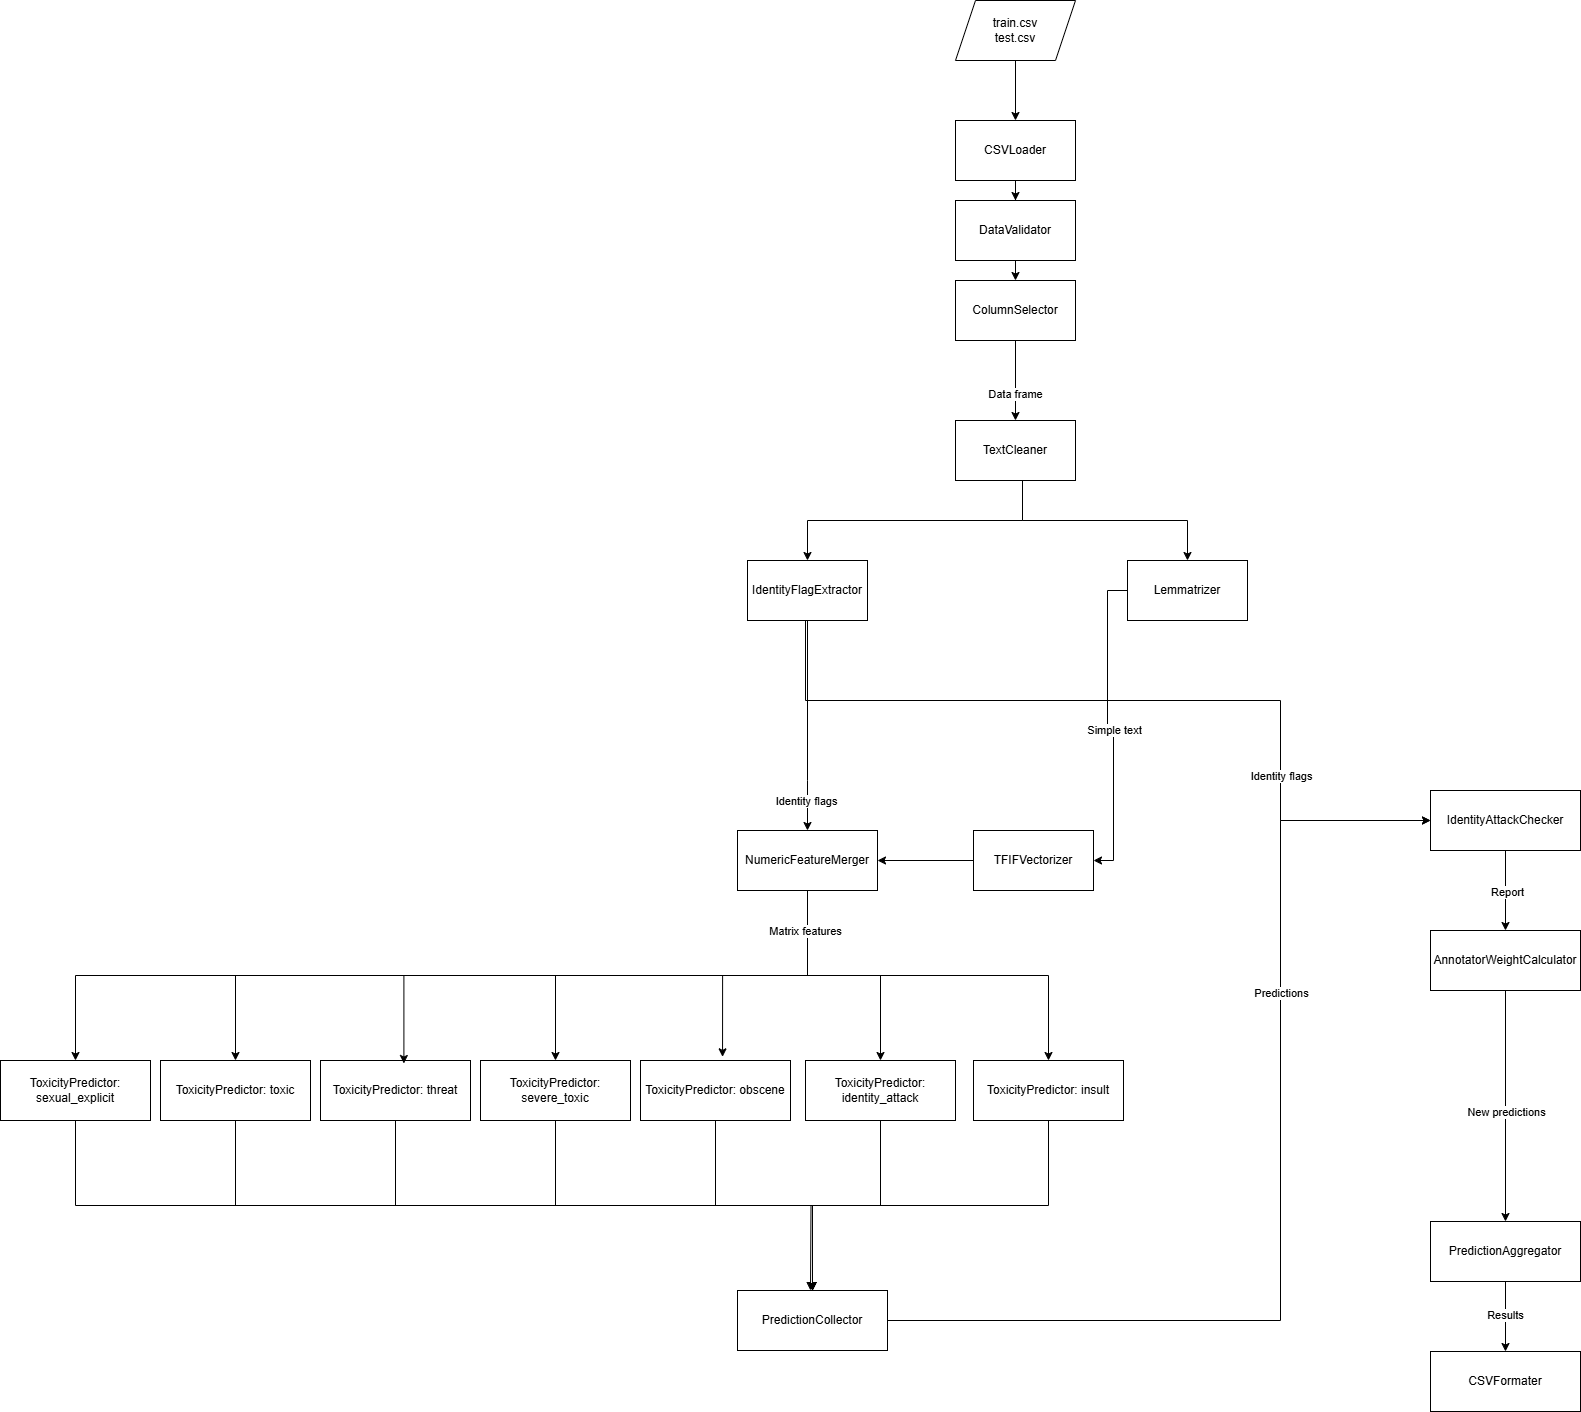
\includegraphics[width=9cm]{img/Systemblueprint.drawio (1).png}\\[0.5cm]



\subsection{Labels:}

\begin{itemize}
\item \textbf{VSCLoader:}: Has the responsibility for extraction. It extracts the data from the files.
\item \textbf{DataValidator}: Has the responsibility to validate the data, that the key columns exist.
\item \textbf{ColumnSelector}: Transforms the received data by removing the columns that are not relevant.
\item \textbf{ColumnSelector}: Transforms the received data by removing the columns that are not relevant.
\item \textbf{TextCleaner}:Transforms the received data by removing the text noise
\item \textbf{IdentityFlagExtractor}: Transforms the identities it detects as a vector
\item \textbf{Lemmatizer}: Transforms the received data by a more simplified text.
\item \textbf{TFIDVectorizer}: Transforms the input text to a vector
\item \textbf{NumericFeatureMerger}: Transforms the input vectors to a matrix, stored in a dataframe
\item \textbf{ToxicityPredictor(X)}:runs an individual model for toxicity prediction
\item \textbf{PredictorCollector}:Transforms each individual prediction, leaving a single dataframe 
\item \textbf{IdentityAttackChecker}: Validates if there are false positives in the identities
\item \textbf{AnnotatorWeightCalculator}: Transforms the possible false positive to a better prediction
\item \textbf{PredictionAggregator}: validates if there are any possible inconsistencies in the final prediction
\item \textbf{CVSFormatter}: outputs in the format required by Kaggle
\end{itemize}
\subsection{System engineering principles}
Designing the system encapsulated in modules makes it scalable because by dividing it into parts it can be developed, modified and maintained without affecting other modules, for example, if we wanted to change the use of TF-ID used to vectorize by BERT none of the other modules would be affected. In addition, modularity also leads to other principles, such as minimal coupling, which is well developed by having modules that communicate only through DataFrames, for example the IdentityAttackChecker only needs the predictions and identities, it is not necessary to know the internal functionality.
\section{Considerations on Chaos and Complexity}
In the context of the systemic analysis we conducted on the Jigsaw Unintended Bias in Toxicity Classification competition, various chaotic and complex elements were identified, stemming from the subjective nature of the data and the processing environment.
\subsection{Chaos in the System}
From a theoretical perspective, the chaos in this system arises primarily from human subjectivity when performing toxicity annotations. The fact that the target value is derived from a fraction of annotators who consider a comment toxic introduces heightened sensitivity to small variations in individual perceptions. Ambiguous, ironic, or sarcastic comments can be interpreted in opposite ways by different annotators, generating a chaotic dynamic that directly impacts the trained model. 
\subsection{Chaos Management Model}
To model this sensitivity and inherent chaos in the system, we have considered the use of two specific classes that encapsulate the main concepts for handling some situations that may arise:
\begin{itemize}
\item \textbf{IdentityAttackChecker}: This class aims to identify subtle or implicit patterns of attacks against identity groups, considering the high variability in how these are perceived. It focuses on identifying cases in which language can have a negative impact, although not always explicitly. This helps capture signals that, although weak, can be amplified in the presence of bias.
\item \textbf{AnnotatorWeightCalculator}: Since not all annotators contribute equally to the evaluation, this class focuses on modeling the influence (or weight) of each one on the final result. Factors such as their tendency to classify more comments as toxic or their bias toward certain identity groups can be quantified and used to adjust the final target value. This allows for the introduction of "dynamic weighting" logic that captures some of the chaotic and nondeterministic behavior of human annotations.
\end{itemize}
\subsection{Nonlinear Behavior and Feedback}
The system also exhibits nonlinear behavior, for example, when small variations in identity scores (such as black = 0.49 vs. black = 0.51) can significantly influence how the model predicts toxicity due to activation functions and decision thresholds. Furthermore, training the model with labels affected by biases can feedback the system if these patterns are not properly detected and mitigated.
These situations can lead to bifurcations in the model's results, where minimal changes in the data or its interpretation generate completely different trajectories in the system's output. Consequently, the introduction of mechanisms such as those mentioned above (IdentifyAttackChecker, AnnotatorWeightCalculator) is essential to mitigate these effects and improve the model's robustness and fairness.

\section{Technologies Used and Implementation Framework}
For the development and implementation of the proposed system, the Python programming language was chosen as the fundamental foundation due to its versatility, clear syntax, and large ecosystem of scientific libraries. This decision was consistent with the management of structured data, the need to perform statistical analysis, and the ease of implementing machine learning models in a modular and transparent manner.
\subsection{Technology Stack}
\begin{itemize}
\item \textbf{Language}: Python (selected for AI/ML ecosystem and Kaggle compatibility)
\item \textbf{Key Libraries}:
\begin{itemize}
\item NumPy: It would be used to solve low-level mathematical operations, especially vector and matrix manipulation. It is essential in the weight calculation phases, operations on feature vectors, and numerical sensitivity assessments.
\item Pandas: It would facilitate the loading, inspection, and transformation of the train.csv, test.csv, and individual annotation files. It would allow us to apply filters, group data by identities, and prepare balanced training sets.
\item Scikit-learn: It would be primarily used to implement linear regression models, such as logistic regression, which act as base models. These models allow for a clearer interpretation of the coefficients associated with each input variable (such as words or tokens) and are useful for evaluating the influence of different features on toxicity prediction.
\end{itemize}
\end{itemize}

\subsection{Modeling Strategy}
The modeling approach was initially based on regression models due to their simplicity and transparency. This allowed us to:
\begin{itemize}
\item Understand how different features (e.g., keywords or identities mentioned) influence the likelihood of a comment being considered toxic.
\item Evaluate the model's behavior in terms of sensitivity to small changes in the data, which is especially relevant considering the presence of chaotic elements in the system.
\end{itemize}
These models were integrated into a modular framework, designed with software and systems engineering principles and focused on scalability and maintainability. The defined modules are:
\begin{itemize}
\item Data Ingestion Module: This module would be responsible for loading the original CSV files, managing formats, and ensuring the integrity of the input data.
\item Preprocessing Module: This module applies text cleansing, normalization, tokenization, and transformation of text into vectors using TF-IDF or other techniques.
\item Modeling and Evaluation Module: In this module, the regression models are trained and evaluated using traditional metrics (AUC, F1-score) and specific fairness metrics such as Subgroup AUC, BPSN AUC, and BNSP AUC.
\item Chaos and Sensitivity Module: The IdentifyAttackChecker and AnnotatorWeightCalculator classes are introduced. These classes would allow us to monitor unstable patterns and adjust weights based on the observed behavior of the annotators, contributing to the stability and fairness of the model. This ensures that unexpected situations do not affect the model if they occur.
\end{itemize}
\section{Conclusion}
This set of technologies would not only be the most appropriate for the proposed challenge but would also allow for agile, reproducible, and easily auditable development, aspects that were highlighted as fundamental in the systemic analysis conducted in the first workshop. The transparency of the stack allows for a better assessment of the impact of decisions on model behavior and facilitates the incorporation of mechanisms to mitigate chaos and excessive sensitivity in the system.

\end{document}